% \tikzset{every picture/.style={line width=0.75pt}} %set default line width to 0.75pt       
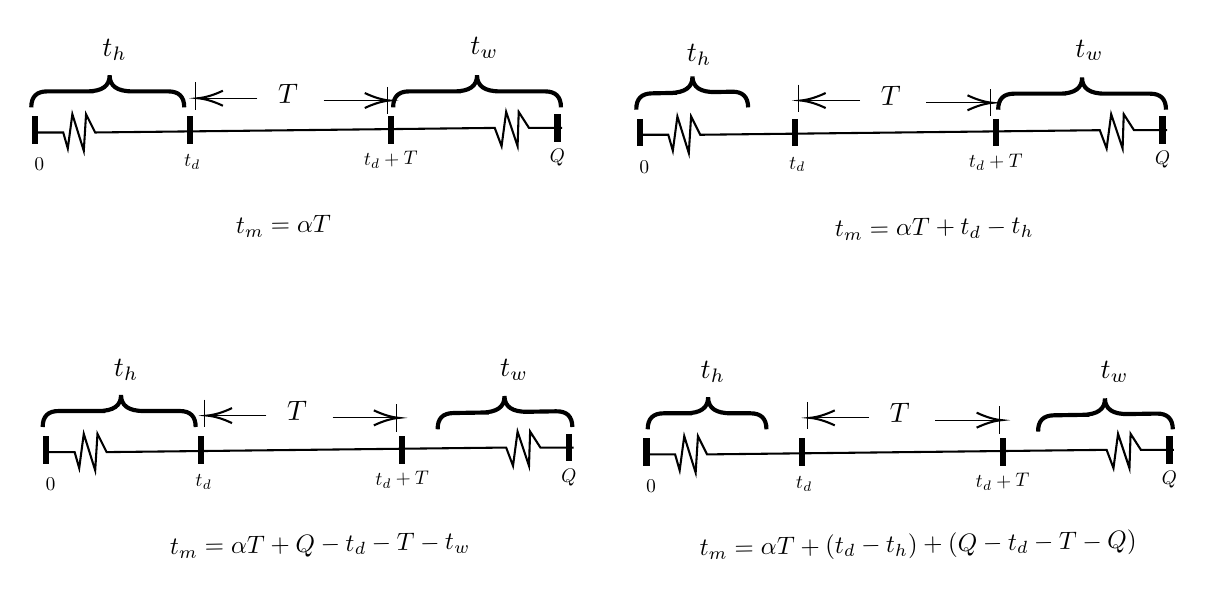
\begin{tikzpicture}[x=0.75pt,y=0.75pt,yscale=-1,xscale=1, scale=1.1]
%uncomment if require: \path (0,262); %set diagram left start at 0, and has height of 262

%Shape: Brace [id:dp6169517089591515] 
\draw  [line width=1.5]  (78.5,46) .. controls (78.5,41.33) and (76.17,39) .. (71.5,39) -- (55.82,39) .. controls (49.15,39) and (45.82,36.67) .. (45.82,32) .. controls (45.82,36.67) and (42.49,39) .. (35.82,39)(38.82,39) -- (18.5,39) .. controls (13.83,39) and (11.5,41.33) .. (11.5,46) ;
%Shape: Brace [id:dp4131205777115946] 
\draw  [line width=1.5]  (243.5,46) .. controls (243.5,41.33) and (241.17,39) .. (236.5,39) -- (216.75,39) .. controls (210.08,39) and (206.75,36.67) .. (206.75,32) .. controls (206.75,36.67) and (203.42,39) .. (196.75,39)(199.75,39) -- (177,39) .. controls (172.33,39) and (170,41.33) .. (170,46) ;
%Straight Lines [id:da38667449766519557] 
\draw [color={rgb, 255:red, 0; green, 0; blue, 0 }  ,draw opacity=1 ][line width=0.75]    (244,55) -- (229.5,55) -- (225,48) -- (224.5,63) -- (219.5,48) -- (217.5,63) -- (214.5,55) -- (39.5,57) -- (35.5,49) -- (34.5,65) -- (29.5,49) -- (27.5,64) -- (25.5,57) -- (14,57) ;


%Straight Lines [id:da7437120864039053] 
\draw [line width=2.25]    (13,50) -- (13,62) ;


%Straight Lines [id:da34292863475953517] 
\draw [line width=2.25]    (81,50) -- (81,62) ;


%Straight Lines [id:da21717714518989284] 
\draw [line width=2.25]    (169,50) -- (169,62) ;


%Straight Lines [id:da8184808038203972] 
\draw [line width=2.25]    (242,49) -- (242,61) ;


%Shape: Brace [id:dp5092713193701387] 
\draw  [line width=1.5]  (83.5,186) .. controls (83.5,181.33) and (81.17,179) .. (76.5,179) -- (60.82,179) .. controls (54.15,179) and (50.82,176.67) .. (50.82,172) .. controls (50.82,176.67) and (47.49,179) .. (40.82,179)(43.82,179) -- (23.5,179) .. controls (18.83,179) and (16.5,181.33) .. (16.5,186) ;
%Shape: Brace [id:dp3077967093237889] 
\draw  [line width=1.5]  (248.5,186) .. controls (248.42,181.33) and (246.05,179.04) .. (241.38,179.12) -- (228.88,179.33) .. controls (222.21,179.44) and (218.84,177.17) .. (218.76,172.5) .. controls (218.84,177.17) and (215.55,179.56) .. (208.88,179.67)(211.88,179.62) -- (196.38,179.88) .. controls (191.71,179.96) and (189.42,182.33) .. (189.5,187) ;
%Straight Lines [id:da9559839515457479] 
\draw [color={rgb, 255:red, 0; green, 0; blue, 0 }  ,draw opacity=1 ][line width=0.75]    (249,195) -- (234.5,195) -- (230,188) -- (229.5,203) -- (224.5,188) -- (222.5,203) -- (219.5,195) -- (44.5,197) -- (40.5,189) -- (39.5,205) -- (34.5,189) -- (32.5,204) -- (30.5,197) -- (19,197) ;


%Straight Lines [id:da8846366028515129] 
\draw [line width=2.25]    (18,190) -- (18,202) ;


%Straight Lines [id:da5600320533816161] 
\draw [line width=2.25]    (86,190) -- (86,202) ;


%Straight Lines [id:da8585404099895867] 
\draw [line width=2.25]    (174,190) -- (174,202) ;


%Straight Lines [id:da1984220618212268] 
\draw [line width=2.25]    (247,189) -- (247,201) ;


%Shape: Brace [id:dp2465407228834131] 
\draw  [line width=1.5]  (325.5,46) .. controls (325.41,41.33) and (323.03,39.05) .. (318.36,39.14) -- (311.23,39.29) .. controls (304.56,39.42) and (301.18,37.16) .. (301.09,32.5) .. controls (301.18,37.16) and (297.9,39.56) .. (291.23,39.7)(294.23,39.64) -- (283.36,39.86) .. controls (278.69,39.95) and (276.41,42.33) .. (276.5,47) ;
%Shape: Brace [id:dp9693935205637665] 
\draw  [line width=1.5]  (508.5,47) .. controls (508.5,42.33) and (506.17,40) .. (501.5,40) -- (481.75,40) .. controls (475.08,40) and (471.75,37.67) .. (471.75,33) .. controls (471.75,37.67) and (468.42,40) .. (461.75,40)(464.75,40) -- (442,40) .. controls (437.33,40) and (435,42.33) .. (435,47) ;
%Straight Lines [id:da5449891341194785] 
\draw [color={rgb, 255:red, 0; green, 0; blue, 0 }  ,draw opacity=1 ][line width=0.75]    (509,56) -- (494.5,56) -- (490,49) -- (489.5,64) -- (484.5,49) -- (482.5,64) -- (479.5,56) -- (304.5,58) -- (300.5,50) -- (299.5,66) -- (294.5,50) -- (292.5,65) -- (290.5,58) -- (279,58) ;


%Straight Lines [id:da471736628836651] 
\draw [line width=2.25]    (278,51) -- (278,63) ;


%Straight Lines [id:da6698452318226781] 
\draw [line width=2.25]    (346,51) -- (346,63) ;


%Straight Lines [id:da0949189707071676] 
\draw [line width=2.25]    (434,51) -- (434,63) ;


%Straight Lines [id:da3498755158637674] 
\draw [line width=2.25]    (507,50) -- (507,62) ;


%Shape: Brace [id:dp9877066436718864] 
\draw  [line width=1.5]  (333.5,187) .. controls (333.5,182.33) and (331.17,180) .. (326.5,180) -- (317.95,180) .. controls (311.28,180) and (307.95,177.67) .. (307.95,173) .. controls (307.95,177.67) and (304.62,180) .. (297.95,180)(300.95,180) -- (288.5,180) .. controls (283.83,180) and (281.5,182.33) .. (281.5,187) ;
%Shape: Brace [id:dp07582394116027302] 
\draw  [line width=1.5]  (511.5,187) .. controls (511.42,182.33) and (509.05,180.04) .. (504.38,180.12) -- (491.88,180.33) .. controls (485.21,180.44) and (481.84,178.17) .. (481.76,173.5) .. controls (481.84,178.17) and (478.55,180.56) .. (471.88,180.67)(474.88,180.62) -- (459.38,180.88) .. controls (454.71,180.96) and (452.42,183.33) .. (452.5,188) ;
%Straight Lines [id:da2560412051217885] 
\draw [color={rgb, 255:red, 0; green, 0; blue, 0 }  ,draw opacity=1 ][line width=0.75]    (512,196) -- (497.5,196) -- (493,189) -- (492.5,204) -- (487.5,189) -- (485.5,204) -- (482.5,196) -- (307.5,198) -- (303.5,190) -- (302.5,206) -- (297.5,190) -- (295.5,205) -- (293.5,198) -- (282,198) ;


%Straight Lines [id:da8821193631068991] 
\draw [line width=2.25]    (281,191) -- (281,203) ;


%Straight Lines [id:da847629160102902] 
\draw [line width=2.25]    (349,191) -- (349,203) ;


%Straight Lines [id:da49564473284443433] 
\draw [line width=2.25]    (437,191) -- (437,203) ;


%Straight Lines [id:da8992381817368192] 
\draw [line width=2.25]    (510,190) -- (510,202) ;


%Straight Lines [id:da9509814866581403] 
\draw    (139.5,43) -- (166.5,43) ;
\draw [shift={(168.5,43)}, rotate = 180] [color={rgb, 255:red, 0; green, 0; blue, 0 }  ][line width=0.75]    (10.93,-3.29) .. controls (6.95,-1.4) and (3.31,-0.3) .. (0,0) .. controls (3.31,0.3) and (6.95,1.4) .. (10.93,3.29)   ;

%Straight Lines [id:da9068324946769639] 
\draw    (167.5,37) -- (167.5,49) ;



%Straight Lines [id:da6523857152326479] 
\draw    (110.5,42) -- (86.5,42) ;
\draw [shift={(84.5,42)}, rotate = 360] [color={rgb, 255:red, 0; green, 0; blue, 0 }  ][line width=0.75]    (10.93,-3.29) .. controls (6.95,-1.4) and (3.31,-0.3) .. (0,0) .. controls (3.31,0.3) and (6.95,1.4) .. (10.93,3.29)   ;

%Straight Lines [id:da9465200262807603] 
\draw    (83.5,35) -- (83.5,47) ;




%Straight Lines [id:da4758380834081246] 
\draw    (403.5,44) -- (430.5,44) ;
\draw [shift={(432.5,44)}, rotate = 180] [color={rgb, 255:red, 0; green, 0; blue, 0 }  ][line width=0.75]    (10.93,-3.29) .. controls (6.95,-1.4) and (3.31,-0.3) .. (0,0) .. controls (3.31,0.3) and (6.95,1.4) .. (10.93,3.29)   ;

%Straight Lines [id:da7287799606206182] 
\draw    (431.5,38) -- (431.5,50) ;



%Straight Lines [id:da21491467191660185] 
\draw    (374.5,43) -- (350.5,43) ;
\draw [shift={(348.5,43)}, rotate = 360] [color={rgb, 255:red, 0; green, 0; blue, 0 }  ][line width=0.75]    (10.93,-3.29) .. controls (6.95,-1.4) and (3.31,-0.3) .. (0,0) .. controls (3.31,0.3) and (6.95,1.4) .. (10.93,3.29)   ;

%Straight Lines [id:da9839139965261974] 
\draw    (347.5,36) -- (347.5,48) ;




%Straight Lines [id:da14148127239163077] 
\draw    (143.5,182) -- (170.5,182) ;
\draw [shift={(172.5,182)}, rotate = 180] [color={rgb, 255:red, 0; green, 0; blue, 0 }  ][line width=0.75]    (10.93,-3.29) .. controls (6.95,-1.4) and (3.31,-0.3) .. (0,0) .. controls (3.31,0.3) and (6.95,1.4) .. (10.93,3.29)   ;

%Straight Lines [id:da5186351191879346] 
\draw    (171.5,176) -- (171.5,188) ;



%Straight Lines [id:da9731173591957024] 
\draw    (114.5,181) -- (90.5,181) ;
\draw [shift={(88.5,181)}, rotate = 360] [color={rgb, 255:red, 0; green, 0; blue, 0 }  ][line width=0.75]    (10.93,-3.29) .. controls (6.95,-1.4) and (3.31,-0.3) .. (0,0) .. controls (3.31,0.3) and (6.95,1.4) .. (10.93,3.29)   ;

%Straight Lines [id:da8230542073493375] 
\draw    (87.5,174) -- (87.5,186) ;




%Straight Lines [id:da5076243934609079] 
\draw    (407.5,183) -- (434.5,183) ;
\draw [shift={(436.5,183)}, rotate = 180] [color={rgb, 255:red, 0; green, 0; blue, 0 }  ][line width=0.75]    (10.93,-3.29) .. controls (6.95,-1.4) and (3.31,-0.3) .. (0,0) .. controls (3.31,0.3) and (6.95,1.4) .. (10.93,3.29)   ;

%Straight Lines [id:da7861981715712135] 
\draw    (435.5,177) -- (435.5,189) ;



%Straight Lines [id:da7294447234655764] 
\draw    (378.5,182) -- (354.5,182) ;
\draw [shift={(352.5,182)}, rotate = 360] [color={rgb, 255:red, 0; green, 0; blue, 0 }  ][line width=0.75]    (10.93,-3.29) .. controls (6.95,-1.4) and (3.31,-0.3) .. (0,0) .. controls (3.31,0.3) and (6.95,1.4) .. (10.93,3.29)   ;

%Straight Lines [id:da862652611937099] 
\draw    (351.5,175) -- (351.5,187) ;





% Text Node
\draw (48,21) node [color={rgb, 255:red, 179; green, 35; blue, 24 }  ,opacity=1 ,rotate=-358.7]  {$\textcolor[rgb]{0,0,0}{t}\textcolor[rgb]{0,0,0}{_{h}}$};
% Text Node
\draw (15,71) node [scale=0.7,color={rgb, 255:red, 0; green, 0; blue, 0 }  ,opacity=1 ,rotate=-358.7]  {$0$};
% Text Node
\draw (82,70) node [scale=0.7,color={rgb, 255:red, 0; green, 0; blue, 0 }  ,opacity=1 ,rotate=-358.7]  {$t_{d}$};
% Text Node
\draw (169,69) node [scale=0.7,color={rgb, 255:red, 0; green, 0; blue, 0 }  ,opacity=1 ,rotate=-358.7]  {$t_{d} +T$};
% Text Node
\draw (242,68) node [scale=0.7,color={rgb, 255:red, 0; green, 0; blue, 0 }  ,opacity=1 ,rotate=-358.7]  {$Q$};
% Text Node
\draw (210,20) node [color={rgb, 255:red, 179; green, 35; blue, 24 }  ,opacity=1 ,rotate=-358.7]  {$\textcolor[rgb]{0,0,0}{t}\textcolor[rgb]{0,0,0}{_{w}}$};
% Text Node
\draw (122,98) node [scale=0.9,color={rgb, 255:red, 0; green, 0; blue, 0 }  ,opacity=1 ,rotate=-359]  {$t_{m} =\alpha T$};
% Text Node
\draw (53,161) node [color={rgb, 255:red, 179; green, 35; blue, 24 }  ,opacity=1 ,rotate=-358.7]  {$\textcolor[rgb]{0,0,0}{t}\textcolor[rgb]{0,0,0}{_{h}}$};
% Text Node
\draw (20,211) node [scale=0.7,color={rgb, 255:red, 0; green, 0; blue, 0 }  ,opacity=1 ,rotate=-358.7]  {$0$};
% Text Node
\draw (87,210) node [scale=0.7,color={rgb, 255:red, 0; green, 0; blue, 0 }  ,opacity=1 ,rotate=-358.7]  {$t_{d}$};
% Text Node
\draw (174,209) node [scale=0.7,color={rgb, 255:red, 0; green, 0; blue, 0 }  ,opacity=1 ,rotate=-358.7]  {$t_{d} +T$};
% Text Node
\draw (247,208) node [scale=0.7,color={rgb, 255:red, 0; green, 0; blue, 0 }  ,opacity=1 ,rotate=-358.7]  {$Q$};
% Text Node
\draw (223,161) node [color={rgb, 255:red, 179; green, 35; blue, 24 }  ,opacity=1 ,rotate=-358.7]  {$\textcolor[rgb]{0,0,0}{t}\textcolor[rgb]{0,0,0}{_{w}}$};
% Text Node
\draw (138,238) node [scale=0.9,color={rgb, 255:red, 0; green, 0; blue, 0 }  ,opacity=1 ,rotate=-359]  {$t_{m} =\alpha T+Q-t_{d} -T-t_{w}$};
% Text Node
\draw (304,23) node [color={rgb, 255:red, 179; green, 35; blue, 24 }  ,opacity=1 ,rotate=-358.7]  {$\textcolor[rgb]{0,0,0}{t}\textcolor[rgb]{0,0,0}{_{h}}$};
% Text Node
\draw (280,72) node [scale=0.7,color={rgb, 255:red, 0; green, 0; blue, 0 }  ,opacity=1 ,rotate=-358.7]  {$0$};
% Text Node
\draw (347,71) node [scale=0.7,color={rgb, 255:red, 0; green, 0; blue, 0 }  ,opacity=1 ,rotate=-358.7]  {$t_{d}$};
% Text Node
\draw (434,70) node [scale=0.7,color={rgb, 255:red, 0; green, 0; blue, 0 }  ,opacity=1 ,rotate=-358.7]  {$t_{d} +T$};
% Text Node
\draw (507,69) node [scale=0.7,color={rgb, 255:red, 0; green, 0; blue, 0 }  ,opacity=1 ,rotate=-358.7]  {$Q$};
% Text Node
\draw (475,21) node [color={rgb, 255:red, 179; green, 35; blue, 24 }  ,opacity=1 ,rotate=-358.7]  {$\textcolor[rgb]{0,0,0}{t}\textcolor[rgb]{0,0,0}{_{w}}$};
% Text Node
\draw (407,99) node [scale=0.9,color={rgb, 255:red, 0; green, 0; blue, 0 }  ,opacity=1 ,rotate=-359]  {$t_{m} =\alpha T+t_{d} -t_{h}$};
% Text Node
\draw (310,162) node [color={rgb, 255:red, 179; green, 35; blue, 24 }  ,opacity=1 ,rotate=-358.7]  {$\textcolor[rgb]{0,0,0}{t}\textcolor[rgb]{0,0,0}{_{h}}$};
% Text Node
\draw (283,212) node [scale=0.7,color={rgb, 255:red, 0; green, 0; blue, 0 }  ,opacity=1 ,rotate=-358.7]  {$0$};
% Text Node
\draw (350,211) node [scale=0.7,color={rgb, 255:red, 0; green, 0; blue, 0 }  ,opacity=1 ,rotate=-358.7]  {$t_{d}$};
% Text Node
\draw (437,210) node [scale=0.7,color={rgb, 255:red, 0; green, 0; blue, 0 }  ,opacity=1 ,rotate=-358.7]  {$t_{d} +T$};
% Text Node
\draw (510,209) node [scale=0.7,color={rgb, 255:red, 0; green, 0; blue, 0 }  ,opacity=1 ,rotate=-358.7]  {$Q$};
% Text Node
\draw (486,162) node [color={rgb, 255:red, 179; green, 35; blue, 24 }  ,opacity=1 ,rotate=-358.7]  {$\textcolor[rgb]{0,0,0}{t}\textcolor[rgb]{0,0,0}{_{w}}$};
% Text Node
\draw (400,238) node [scale=0.9,color={rgb, 255:red, 0; green, 0; blue, 0 }  ,opacity=1 ,rotate=-359]  {$t_{m} =\alpha T+( t_{d} -t_{h}) +( Q-t_{d} -T-Q)$};
% Text Node
\draw (124,40) node [color={rgb, 255:red, 0; green, 0; blue, 0 }  ,opacity=1 ,rotate=-358.7]  {$T$};
% Text Node
\draw (388,41) node [color={rgb, 255:red, 0; green, 0; blue, 0 }  ,opacity=1 ,rotate=-358.7]  {$T$};
% Text Node
\draw (128,179) node [color={rgb, 255:red, 0; green, 0; blue, 0 }  ,opacity=1 ,rotate=-358.7]  {$T$};
% Text Node
\draw (392,180) node [color={rgb, 255:red, 0; green, 0; blue, 0 }  ,opacity=1 ,rotate=-358.7]  {$T$};


\end{tikzpicture}
